\documentclass{standalone}
\usepackage{tikz}
\usepackage{ctex,siunitx}
\setCJKmainfont{Noto Serif CJK SC}
\usepackage{tkz-euclide}
\usepackage{amsmath}
\usetikzlibrary{patterns, calc,3d}
\usetikzlibrary {decorations.pathmorphing,decorations.pathreplacing,decorations.shapes}
\tikzset{label style/.append style={font=\small}}
\begin{document}
\small
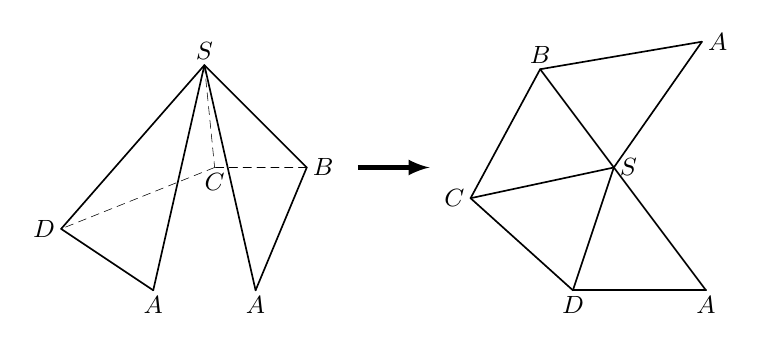
\begin{tikzpicture}[>=latex,scale=1.3,inner sep=2pt]
  \begin{scope}
    \tkzDefPoints{0/0/S,0.9/-1.2/A,-0.4/-1.2/D,-1.4/-0.3/C,-0.72/0.96/B}
    \tkzDefShiftPoint[S](55:1.5){A'}
    \tkzDrawSegments[semithick](A',B A,D B,C C,D S,A S,B S,C S,D S,A')
    \tkzLabelPoints[right](S)
    \tkzLabelPoint[right](A'){$A$}
    \tkzLabelPoints[left](C)
    \tkzLabelPoints[above](B)
    \tkzLabelPoints(A,D)
  \end{scope}
  \begin{scope}[xshift=-4cm]
    \tkzDefPoints{0/1.0/S,-0.5/-1.2/A,-1.4/-0.6/D,0.1/0/C,1.0/0/B,0.5/-1.2/A'}
    \tkzDrawSegments[semithick](A',B A,D S,A S,B S,D S,A')
    \tkzDrawSegments[densely dashed](S,C B,C C,D)
    \tkzLabelPoints[above](S)
    \tkzLabelPoint[below](A'){$A$}
    \tkzLabelPoints(A,C)
    \tkzLabelPoints[left](D)
    \tkzLabelPoints[right](B)
  \end{scope}
  \draw[ultra thick,->](-2.5,0)--++(0.7,0);
\end{tikzpicture}
\end{document}